\documentclass[12pt,a4paper]{article}



\usepackage{multirow}
\usepackage[normalem]{ulem}
\useunder{\uline}{\ul}{}
\usepackage{caption}

\usepackage[T1]{fontenc} % Font encoding (e.g. hyphenation w/ accented characters)
\usepackage[utf8]{inputenc} % utf-8 support
\usepackage[english]{babel} % English as main language 
\addto\captionsenglish{\renewcommand{\contentsname}{Table of Contents}} % after babel 
\usepackage{kpfonts}

\usepackage{graphicx} % graphics
\graphicspath{{Graphics/}{../Graphics/}} % path to Graphics
\usepackage[bookmarksdepth=3,pdfpagelayout=TwoPageRight,
pdftoolbar=false,hyperfootnotes=false,
pdfpagelabels=true]{hyperref}
\usepackage{color} 
\definecolor{utblue}{RGB}{10,90,200} % from color-package
%\hypersetup{colorlinks=true,linkcolor=utblue,urlcolor=utblue}
\hypersetup{colorlinks=true,linkcolor=black,citecolor=black,urlcolor=black}
\usepackage[margin=25mm]{geometry}
\usepackage{longtable}
%\linespread{1.5}
\renewcommand{\baselinestretch}{1.3} % ~ 1.5 line spacing
%\usepackage[parfill]{parskip} % space between parag. instead of indent
\setlength{\parskip}{2pt} % "subtle" space between parag.
%\usepackage{sectsty} % section formatting (section style)
%\sectionfont{\LARGE} % font size of section
%\subsectionfont{\Large} % font size of subsection
%\subsubsectionfont{\large} % font size of subsubsection
%\paragraphfont{\large} % font size of subsubsection
%\setcounter{secnumdepth}{4}

%% Penalties
\widowpenalty=10000 % no single lines at the top of a page
\clubpenalty=10000 % no single lines at the end of a page
\displaywidowpenalty=10000 % \widowpenalty im "math mode"
\interfootnotelinepenalty=10000 % footnotes always on one page
% fine tuning: \looseness+1 or \looseness-1 before \par

%% Math
\usepackage{amsfonts,amsmath,amssymb,mathrsfs} % math. symbols
\allowdisplaybreaks % subequations across more than one page
%\usepackage{physics} % use of \pdv{}{} for partial derivatives % second partial derivative \pdv[n]{Q}{t}

%% Footnotes
\usepackage{setspace} % 1.5 line spacing not for footnotes
\setstretch{1.5}
\setlength{\footnotesep}{10pt} % some space between footnotes
\usepackage[multiple,bottom]{footmisc} % footnotes always at bottom

%% Citation

\usepackage{natbib} % formatting citation and bibliography
\renewcommand{\cite}{\citet} % [page] as option 
%\hypersetup{citecolor=utblue}
%\setcitestyle{notesep={, page }}

%% Tables
\usepackage{tabu} % tabu-environment, \tabulinesep
\usepackage{booktabs} % horizontal lines in tables, usage with \toprule, \midrule, \bottomrule
%\usepackage{float} % determining the position of e.g. tables
\usepackage[font=small,labelfont=bf]{caption} % formatting of captions

%% Misc
\usepackage{subcaption} % for subfigure-environment
\usepackage{bookmark} % corrects hyperlinks in pdf-file
\usepackage{lipsum} % dummy text for template

%% New commands
\newcommand{\R}{{\mathbb R}}
\newcommand{\N}{\mathcal{N}}
\newcommand{\E}{\mathrm{E}}			
\newcommand{\Lg}{\mathcal{L}} % lagrangian L
\newcommand{\Var}{\mathrm{Var}}
\newcommand{\Cov}{\mathrm{Cov}}
\newcommand{\Corr}{\mathrm{Corr}}

\usepackage[capposition=top]{floatrow}

%% Suggested/additional/optional packages
%\usepackage{tocloft} % additional TOC options
%\usepackage{etoc} % local TOCs
%\usepackage{pdfpages} % \includepdf[pages={1-},scale=1]{*.pdf}
%\usepackage{etoolbox} % tool to "patch" the commands
%\usepackage{tikz} % simple graphics with TikZ
%\usepackage{tikzscale} % scales on page width
%\usepackage{filecontents} % imports TikZ as figures
%\usepackage{svg} % vector graphics
%\usepackage{longtable} % tables with page break
%\usepackage{bookmark} % corrects hyperlinks in pdf-file
%\usepackage[normalem]{ulem} % strikethrough and cancel out
%\usepackage{microtype} % to get more compact text, reduces grey part
%\usepackage{csquotes} % selects quotation marks automatically depending on the selected language
%\usepackage[abbreviations,british]{foreign} % correct spacing for abbreviations, e.g. e.g.
%\usepackage{lscape} % \begin{landscape} for a single or multiple horizontal pages
	
	
	\begin{document}
		\begin{titlepage}\label{sec:title}\newgeometry{margin=30mm}	
			\begin{center}
				{\huge \bfseries \hrulefill\\
					Semi-parametric Estimation of a Heterogeneous Intermediaries Stochastic Discount Factor\\
					\hrulefill}\\[4mm]
				{\Large \bfseries
					Seminar Paper\\[12mm]
					
					Janik Müller}\\
				Charlottenstraße 8\\
				72070 Tübingen\\
				Matrikel-Nr.: 6303477\\[10mm] 
				{\large 
					Eberhard Karls Universität Tübingen\\[2mm]
					Supervisor: \\
					Prof. Dr. Joachim Grammig, \\
					M.Sc. Alexander Reining  \\[2mm]
					Submission: \today}
			\end{center}
			\clearpage\thispagestyle{empty}\mbox{} % blank page
		\end{titlepage}\restoregeometry	
		
		% --- start page numbering ---	
		\tableofcontents
		\clearpage
		%
		
		
\section{Introduction}

%What should be answered here: \\
%- What is the problem? \\
%- Why is it important? \\
%- What is my approach? \\
%- What are the key results? \\
%- What papers already talked about this topic? \\
%- What is the structure of the paper? \\
%- What is different between the paper I am re-building on and my paper? \\



A lot of research is currently being done on the impact financial intermediaries have on pricing different asset classes. After the development of the consumption based asset pricing model (CCAPM) by **Citation needed** the focus started to shift onto the role financial intermediates play in this regard. 
The empirical findings of **AEM** and **HKM** where it was discovered that a stochastic discount factor (SDF) that includes the intermediary's balance sheet data possess an intriguing potential in explaining the risk-premia in a cross-section of asset returns. In the aforementioned papers the intermediary sector was assumed to be homogeneous. **Check if this is true!**
However, in reality the intermediary sector is heterogeneous and the balance sheet data of different intermediaries can vary significantly. The paper of **SA MAI** aimed to extend the work on **AEM** and **HKM** by introducing a heterogeneous intermediary stochastic discount factor (HI-SDF) that includes the balance sheet data of two different types of intermediaries. Furthermore, **SA MAI's** paper also incorporated a non-linear functional form for the intermediary's contributions build on top of the established CCAPM model using the power utility of the households. 
Since **SA MAI** uses data up until the COVID-19 pandemic, the aim of this paper is to therefore replicate the results and to further investigate if the estimates and the pricing-abilities of HI-SDF, in the proposed functional form, was in any way affected by the COVID-19 crisis. 
Following the methodology of **SA MAI**, the paper will use a two-step estimation procedure to estimate the parameters of the HI-SDF.
The first step is to estimate the intermediary-specific parameters using the *Sieve minimum distance* and then using these intermediary-specific-estimates in a second step GMM framework to estimate the risk-aversion parameters of the households.

A better understanding of the role and functional form of financial intermediaries in asset pricing may lead to more robustness in the pricing of different securities and may help in determining the absurdly high risk-aversion parameters estimated by CCAPM models throughout the literature.


\newpage


\section{Methodology}

In this section, we will explore the structure of heterogeneous intermediaries and the stochastic discount factor (HI-SDF), as well as its components and their relevance. After theoretically establishing the HI-SDF, we will move on to the two-step semi-parametric estimation procedure, which uses a first-step Sieve Minimum distance approach in order to non-parametrically estimate the infinite-dimensional function $\Omega$ and a second-step General Method of Moments estimation to estimate the preference parameters $\beta$ and $\gamma$ as well as refine the estimation of $\Omega$. Following this discussion, we will then explain the structure of the data used in estimation.

	\subsection{Structure of the HI-SDF}
	
	The HI-SDF builds upon the consumption-based asset pricing model (CCAPM) as a foundational framework. However, it extends and modifies it significantly to incorporate the role of financial intermediaries and their heterogeneity. The HI-SDF retains the core component of the CCAPM, which is households' marginal rate of substitution (MRS). 
	This MRS captures the idea that asset prices reflect the trade-off households make between today's and tomorrow's consumption. In essence, high uncertainty about tomorrow's consumption will result in a higher required return by the investor to hold a risky asset.
	Building on top of this foundation, the HI-SDF introduces a pricing wedge $\Omega(\psi_t, \phi_t)$ that accounts for variations in leverage $(\phi_t)$ and net worth share $(\psi_t)$ across intermediaries. Incorporating these variables allows us to capture the impact financial frictions and intermediary heterogeneity have on asset prices, helping us to build a deeper understanding of risk premia.
	
	The HI-SDF $m_t$ takes, therefore, the following form:
	
	\begin{align}
		m_t = \beta \left( \frac{C_t}{C_{t-1}} \right)^{-\gamma} \Omega(\psi_t, \phi_t)
		\label{m_t}
	\end{align}
	
	
	Where $ \beta \left( \frac{C_t}{C_{t-1}} \right)^{-\gamma} $ captures the households marginal rate of substitution, as is already known from the CCAPM, and $ \Omega(\psi_t, \phi_t) $ is the aforementioned pricing wedge the constitutes as a general function of the net worth share among intermediaries $\psi_t$ and the $\phi_t$ is the aggregate intermediary leverage. 
	
	
	In the literature, the intermediary-specific variables are often present, as in \textbf{Insert paper where this is the case here}, but the functional form of $ \Omega(.) $ remains either unknown or is modeled to be linear in its nature.
	Conversely, in our approach, $ \Omega $ is to be inferred from the data and not explicitly modeled beforehand. Letting the data speak for the functional form of $\Omega(.)$ allows the HI-SDF to incorporate nonlinear dynamics and the heterogeneity between the intermediaries.
	
	



	\subsection{Semiparametric Estimation Procedure and Theory}

	After introducing the HI-SDF and the incorporated pricing wedge $\Omega$ in the chapter before we will now look at the estimation procedure that is used in order to estimate the newly formed HI-SDF. Since we are not imposing any functional structure on $\Omega(.)$ we are left with the challenge following challenge for our estimation: $\Omega(.)$ is unobservable and must therefore be inferred from the observable data. This issue was addressed by Sai Ma (2023) in his paper by following the procedure of \textbf{Chen, Favilukis and Ludvigson (2014)}. They applied the aforementioned two-step sieve minimum distance (SMD) and GMM estimation strategy. Using this procedure requires us to define an appropriate moment condition which is derived below. It has its starting point in the \textit{Euler-Equation} and the general formulation of the HI-SDF in equation (\ref{m_t}). 
	We start with the well known general Euler Equation:
	\begin{align}
	E_t = [m_{t+1} R_{t+1} | \mathcal{F_t}] = 1
	\label{eq:basis_euler}
	\end{align}
	
	where $m_{t+1}$ is the stochastic discount factor, $R_{t+1}$ is the gross return on asset $i$ between time $t$ and $t + 1$ and $E_t$ is the conditional expectation formed at time $t$ using the information $\mathcal{F_t}$ available at time $t$. As is trivial this conditional expectation should be equal to one for a gross return. Now substituting $m_t$ with the HI-SDF formulation and rearranging the equation we arrive at the following moment condition which is at the basis of the empirical analysis:
	\begin{align}
		E_t = \left[ \beta \left( \frac{C_{t+1}}{C_t} \right)^{-\gamma}  \Omega(\psi_{t+1}, \phi_{t+1}) R_{i, t+1} -1 \right] = 0
		\label{eq:basis_euler_hi_sdf}
	\end{align}
	
	as is well known in financial economics this equation (\ref{eq:basis_euler_hi_sdf}) states that, in equilibrium, the conditional expectation of the SDF multiplied by the asset's gross return should be equal to unity, ensuring no arbitrage opportunities.
		
		
		
		\subsubsection{Semiparametric Estimation in Theory}
		
		This section is aimed at introducing the theoretical framework for the estimation process as well as the explain the underlying concepts. 		
		
		We start by letting $\nu = (\beta, \gamma)'$ denote the vector of finite dimensional preference parameters to be estimated and letting $\Omega_t$ be a non-parametrically specified function of net worth share $\psi_{t}$ and aggregate leverage $\phi_{t+1}$. 
		We also define $\kappa_i$ for each test asset $i = 1, ..., N$ as follows:
		\begin{align}
			\kappa_i(\textbf{z}_{t+1}, \nu, \Omega)    \equiv  \beta \left( \frac{C_{t+1}}{C_t} \right)^{-\gamma}  \Omega(\psi_{t+1}, \phi_{t+1}) R_{i, t+1} - 1
			\label{eq:kappa_i}
		\end{align}
		
		where for notional brevity $z_{t+1}$ is a vector of all observations and $\kappa_i(.)$ is the residual between the HI-SDF implied returns and the actually observed returns for all assets $N$ at time $t+1$. This then in turn lets us write the conditional moment condition as follows:
		\begin{align}
			E(\kappa_i(\textbf{z}_{t+1}, \nu, \Omega) | \mathcal{F}_t) = 0 
			\label{eq:model_correctly_specified}
		\end{align}
		
		where $\mathcal{F_t}$ is the set of information available at time $t$ and we can state that the model is correctly specified if the equation holds for all test assets $i \in \{ 1,2,...,N \}$. In that case $\Omega = \Omega_0$ and $\nu = \nu_0$. 
		We define $\Omega_0$ to be the value that minimizes the conditional moment's restriction squared distance from zero, i.e. ensuring that the conditional moment conditions are satisfied as closely as possible. Be aware however, since $\Omega(.)$ and $\nu$ both influence $\kappa_i(\textbf{z}_{t+1}, \nu, \Omega)$, which sits at the center of the moment condition, the solution $\Omega_0(., \nu)$ is parameterized by $\nu$, i.e. for a given $\nu$, the optimal $\Omega_0$ is calculated and if $\nu$ changes, so must the functional form of $\Omega$ to ensure that the moment conditions are still satisfied. 
		We can therefore define the optimal $\Omega_0(\cdot,\nu)$ as follows: 
		\begin{align}
			\Omega_0(\cdot, \nu) \equiv \arg \underset{\Omega}\inf  E \left[ \sum_{i = 1}^{N} (	E(\kappa_i(\textbf{z}_{t+1}, \nu, \Omega) | \mathcal{F}_t)^2 \right]
			\label{eq:omega_0}
		\end{align}
		
		where the inner expectation is the conditional expectation of the residual $\kappa_i$ given the information set $\mathcal{F_t}$ thus ensuring that the moment condition for every test asset is satisfied conditionally on $\mathcal{F_t}$. Furthermore, the outer expectation takes the expectation across the entire data distribution therefore ensuring that the solution for $\Omega_0$ is globally valid. 
		
		If we have $\Omega_0$ given by this definition then we can obtain the true parameter values of $\nu_0$ by minimizing the same squared deviation as before only this time evaluated at the true $\Omega_0(\cdot, \nu)$ this gives us the following formula: 
		\begin{align}
			\nu_0 = \underset{\nu}{\min} E \left[ \sum_{i = 1}^{N} (E( \kappa_i(\textbf{z}_{t+1}, \nu, \Omega_0(\cdot, \nu)) | \mathcal{F}_t))^2 \right]
			\label{eq:nu_0}
		\end{align}
		
		If we now denote the instruments as $\textbf{w}_t$, which is an observable subset of $\mathcal{F}_t$, then equation \ref{eq:model_correctly_specified} implies that the following, now using the true parameter values, also holds:
		\begin{align}
				E(\kappa_i(\textbf{z}_{t+1}, \nu, \Omega) | \textbf{w}_t) = 0
				\label{eq:correct_model}
		\end{align}
		
		in this equation the role of $\textbf{w}_t$ is to capture the exogenous information available at time $t$ and to enforce the moment restrictions by ensuring orthogonality between the residuals $\kappa_i$ and the instruments. In mathematical terms this means: $E[\kappa_i \cdot \textbf{w}_t] = 0$, a fundamental property for consistent estimation and identification in semiparametric and GMM-based models.
		
		We can then also define the conditional mean function as follows:
		\begin{align}
			M (\textbf{w}_t, \nu, \Omega) \equiv E[\kappa (\textbf{z}_{t+1}, \nu, \Omega) | \textbf{w}_t]
			\label{eq:cond_mean_condition}
		\end{align}
		
		where, to emphasize that we have a system of moment conditions, $\kappa = (\kappa_i)_{i=1}^{N}$ is a vector of moment conditions. 
		After inserting this conditional mean function back into equation \ref{eq:omega_0} we can define $\Omega^*$ for any candidate value of preference parameters $\nu$ as follows:
		\begin{align}
			\Omega^* \equiv \underset{\Omega}{\inf} = E [ M(\textbf{w}_t, \nu, \Omega)'  M(\textbf{w}_t, \nu, \Omega)].
			\label{eq:omega_star}
		\end{align}
		
		When the model is then correctly specified we receive $\Omega^* = \Omega_0$. We will therefore in the estimation step estimate $\Omega^*$ using a nonparametrically estimated conditional mean vector $M(\textbf{w}_t, \nu, \Omega)$. This definition of $\Omega^*$ gives us the optimal estimate of $\Omega$ for any given candidate $\nu$ by also minimizing the expected squared deviation of the conditional mean function, which in turn is the conditional mean of the residuals $\kappa$. Minimizing this ensures that $M(\textbf{w}_t, \nu, \Omega^*) \approx 0$, which means that the model predictions (through $\kappa$) align with the data as closely as possible. 
		To estimate the model given by equation \ref{eq:correct_model} we use the aforementioned semiparametric minimum distance procedure that consists out of two steps. First we estimate the unknown function $\Omega^*$ for any infinite-dimensional parameter candidate $\nu$, using the sieve minimum distance approach and in the second step we estiate the preference parameters $\beta$ and $\gamma$ conducting a Generalized Method of Moments (GMM) estimation using the optimal function $\Omega^*$ from the first step. 
		
		Having discussed the underlying theoretical framework on the estimation of the parameters we can also note the following interesting observations. The estimation process is not trivial and rather complex. This is due to multiple factors such as the joint nature of $\nu$ and $\Omega$, i.e. the moment condition depends on $\nu$ and $\Omega$ and estimating $\nu_0$ requires knowing $\Omega_0$ and vice versa. Furthermore, since $\Omega$ is not parameterized in a finite-dimensional space, we need to approximate the function using for example sieve basis functions.
		
		
		
	
	
		\subsubsection{First Step: Sieve Minimum Distance Estimation of $\Omega$}
		
		After having laid out the theoretical foundation in the last chapter we will now turn to the estimation procedure. In this chapter we will discuss the implementation strategy that was used in order to arrive at estimates for $\Omega$.
		Due to $\Omega$ being in infinite-dimensional object, and estimating such a function directly is infeasible, it is approximated by a sequence of finite-dimension sieve functions for each candidate of $\nu$. Sieve functions are a mathematical tool that lets us project a an infinite-dimensional function such as $\Omega$ onto a finite-dimensional space spanned by the basis functions. In our case we use B-splines as basis functions which have a degree of $m = 3$, making them so called cubic splines. Splines, and in our case cubic splines, are specifically designed to approximate smooth, nonlinear relationships. They are piece-wise polynomials which means that they are polynomial functions that take on a specific form (e.g. linear, quadratic, cubic) on a specific, predefined interval. These polynomial functions can change from one interval to another at so called knots, or points at which the polynomial functions connect to each other. Further details on the choice of sieve function and splines are discussed in the \textbf{Appendix}. 
		
		In order to estimate the pricing wedge $\Omega$ it is specifically approximated as follows: 
		\begin{align}
			\Omega^*(\psi_{t}, \phi_t, \nu) \approx \Omega_{K_T}(\cdot, \nu)
			= \alpha_0(\nu) + \sum_{j = 1}^{K_T} \alpha_j(\nu) B_j(\psi_{t}, \phi_t)
			\label{eq:approx_omega}
		\end{align}
	
		where $\{B_j\}$ are the basis functions described earlier and  $\{\alpha_j\}$ are the sieve coefficients dependent on $\nu$, which are to be estimated.
		
		As we have seen in the theoretical chapter before in order to estimate $\Omega$ we need a consistent estimate of the conditional mean vector $M(\textbf{w}_t, \nu, \Omega$ which was defined in \ref{eq:cond_mean_condition}. To achieve this consistent estimator and in turn a consistent estimate of $\Omega$ we will apply the sieve least squares method. Since $M(\textbf{w}_t, \nu, \Omega$ is also infinite-dimensional in its nature due to the fact, that it must assign a value for every possible $\text{w}_t$ in a continuous range, we are also approximating it using basis functions. In our analysis this is done by polynomials of order $J_t$. The non-parametric estimation of $\hat{M}(\text{w}_t, \nu, \Omega)$ done by sieve least squares goes as follows. 
		
		For each fixed ($\nu, \Omega$) we approximate the  $M(\text{w}_t, \nu, \Omega)$ by:
		\begin{align}
			\hat{M}(\textbf{w}_t, \nu, \Omega) \approx    {p^{J_T}}'(\textbf{w}_t) \hat{\alpha}
			\label{eq:M_hat_estimation}
		\end{align}
		
		where $p^{J_T}$ is the vector of basis functions of $\textbf{w}_t$ and $\hat{\alpha}$ are the coefficients that need to be estimated. The $\hat{\alpha}$ are estimated via sieve least squares regression, which minimizes the sum of squared residuals:
		\begin{align}
			\underset{\alpha}{\min} \frac{1}{T} \sum_{t = 1}^{T} (\kappa(\textbf{z}_{t+1}, \nu, \Omega) - {p^{J_T}}'(\textbf{w}_t) \alpha)^2
		\end{align}
	
		The solution to this least squares problem is:
		\begin{align}
			\hat{\alpha} = (P'P)^{-1} P' \kappa
			\label{eq:M_hat_matrix}
		\end{align}
	
		we can then substitute $\alpha$ back into equation \ref{eq:M_hat_estimation} and we get:
		\begin{align}
		\hat{M}(\text{w}_t, \nu, \Omega) \approx    {p^{J_T}}'(\textbf{w}_t (P'P)^{-1} P' \kappa
		\label{eq:m_hat_estimation_2}
		\end{align}
	
		where we can expand the term $P' \kappa$ into a summation and receive:
		\begin{align}
			P' \kappa = \sum_{t = 1}^{T} {p^{J_T}}'(\textbf{w}_t \kappa(\textbf{z}_{t+1}, \nu, \Omega)
		\end{align}
	
		and substituting this relationship into \ref{eq:M_hat_matrix} and rearranging this equation we receive the following sieve least squares estimator of the conditional mean vector that can be used in our analysis:
		\begin{align}
			\hat{M}(\textbf{w}_t, \nu, \Omega) = \left( \sum_{t=1}^{T} \kappa(\textbf{z}_{t+1}, \nu, \Omega)  p^{J_T}(\textbf{w}_t)' (P'P)^{-1} \right)  p^{J_T}(\textbf{w})
			\label{eq:M_HAT_Finals}
		\end{align}
	
		where $P$ is a collection of sequences known basis functions $p^{J_T}(w_1), ..., p^{J_T}(w_T)$ with basis functions $p^{J_T}(\cdot) \equiv (p_{01}, ..., p_{0J_T}$ of order $J_T$.
		
		Now using this estimator for $\hat{M}$ we can then estimate $\hat{\Omega}$ for $\Omega^*$ by incorporating the sample equivalent of equation \ref{eq:omega_star} and we receive the following estimator for $\Omega$:
		\begin{align}
			\hat{\Omega}(\cdot, \nu) = \underset{\Omega_{K_T}}{\min} \frac{1}{T} \sum_{t = 1}^{T} \hat{M}(\textbf{w}_t, \nu, \Omega)' \hat{M}(\textbf{w}_t, \nu, \Omega)
		\end{align}
		
		where we therefore approximate $\hat{\Omega}$ by minimizing over $\Omega_{K_T}$ in order to find the smallest squared deviation of the conditional moment restriction represented by $\hat{M}(\textbf{w}_t, \nu, \Omega)$. 
		
		
		This estimation procedure as is described and derived in this part is, as mentioned at the start done for each candidate of $\nu$. This entails that this estimation procedure is run over a predefined grid of $\beta$  and $\gamma$ values and in the end the $\hat{\Omega}$ is chosen that matches the data closest, i.e. that minimized the weighted quadratic norm of the estimated conditional expectation function.
	
	

		
		\subsubsection{Second Step: GMM Estimation of Preference Parameter $\beta$ and $\gamma$}
	
		In this chapter we will rather quickly take a look at the GMM estimation step. Following the initial estimation of $\hat{\Omega}(\cdot, \nu)$ in the first step, we now want to finalize the estimation of the preference parameters $\nu = (\beta, \gamma)$ using the Hansen (1982) Generalized Method of Moments (GMM). 
		Since this is a well established method we will focus on our use case and how the objective function is defined:
		\begin{align}
			\hat{\nu} = \arg \underset{\nu}{\min} Q_T(\nu)
			\label{eq:objective_func_nu}
		\end{align}
		
		where $Q_t(\nu)$ is defined as the criterion function that is to be minimized using GMM. The criterion function takes the following form:
		\begin{align}
			Q_T(\nu) = \left[ g_T \left( \nu, \hat{\Omega}(\cdot, \nu); y^T \right) \right]' \textbf{W} \left[ g_T \left( \nu, \hat{\Omega}(\cdot, \nu); y^T \right) \right]
			\label{eq:objective_func_gmm}
		\end{align}
		
		where \textbf{W} is a positive, semi-definite weighting matrix, and $\textbf{y}^T$ is the vector of observations including $\textbf{z}_t$ and any chosen measurable function of instrument set $\textbf{w}_t$. The sample moment conditions can be expressed as follows: 
		\begin{align}
			g_T\left(\beta, \gamma \vert \hat{\Omega}, y^T\right) = \frac{1}{T} \sum_{t=1}^T \kappa\left(z_{t+1}, \nu, \hat{\Omega}\right) \otimes y^T.
			\label{eq:mom_cond_gmm}
		\end{align}
		
		It is important to note that in this estimation step the function $\hat{\Omega}$ is not held fixed but is still dependent on the preference parameters $\nu$ and might therefore be optimized further by this GMM framework and thus resulting from this second step are the final estimates not only for the preference parameters $\nu$ but also for $\hat{\Omega}(\cdot, \nu)$.
		Other than in Sai Ma (2023) paper we do not use the inverse of the sample second moment of asset returns as our weighting matrix but keep $ \textbf{W} = \textbf{I}$.
		
		Having estimated the time preference parameter $\hat{\beta}$, the risk-aversion parameter $\hat{\gamma}$ and the pricing wedge $\hat{\Omega}$ we can estimate the HI-SDF as follows:
		\begin{align}
			\hat{m}_t (\hat{\nu}, \hat{\Omega}) = \hat{\beta} \left( \frac{C_t}{C_{t-1}} \right)^{-\hat{\gamma}} \hat{\Omega}(\psi_{t}, \phi_{t}).
			\label{eq:HI_SDF_M_Final_Estimation} 
		\end{align}
		
	
	

	
	\subsection{Data and Variables}
%	
%	What should be answered here:
%	
%	* What data was used?
%	* What are the key variables of the data?
%	* Where is the data from and where can it be found?
%	* Why was this data used?
%	* Which time frame does the data cover?
%	* Instruments talk about the choice of $w_t$
	
	In the following section we will talk about the data that was used in the estimation of HI-SDF. Furthermore, we will also cover the which instruments were used in the estimation process and how the leverage and net worth share data was computed.
	
	We will start by explaining which return data was incorporated into the analysis. The data from He, Kelly and Manela (2017) analysis was used to create all non-equity portfolios and their returns. The data incorporates bonds, sovereign bonds, CDS, Options and commodities beginning in 1970 Q1 until 2012 Q4. However, this data is very sparse and their is not a lot of overlap between the different non-equity assets. We furthermore included four equity portfolios which range from 1970 Q4 until 2024 Q3. These portfolios were obtained from Kenneth French'S Dartmouth data library and include 25 size/book-market sorted, 25 size/operating profitability, 10 lon-run reversal and 25 size/investment portfolios. As a proxy for the risk-free rate a three month T-Bill spanning from 1970 Q1 to 2024 Q3 was used in the analysis. Furthermore, we denote the one-period gross return from $t-1$ to $t$ on asset $i$ as: $R_{i, t}$ and an excess return is defined as: $R^{e} \equiv R_{i,t} - R_{f, t}$ with $R_{f,t}$ being the risk-free rate at time $t$.
	The consumption data that builds the foundation for the preference based pricing model was obtained from the U.S. Department of Commerce, Bureau of Economic Analysis. We used the Real Personal Consumption Expenditures [PCECC96] in billions of chain-weighted 2017 dollars and seasonally adjusted at an annual rate as the basis for our consumption growth data. 
	Furthermore, since during the empirical procedures first steps instruments are used in order to estimate the conditional moment $\hat{M}(\textbf{w}_t, \nu, \hat{\Omega})$, we also include them in this list. The instruments are $\textbf{w}_t = \left[ cay_t, RREL_t, \frac{C_t}{C_{t-1}}, \phi_t \right]'$. Here $cay_t$ stands for the log consumption-wealth ratio studied by Lettau and Ludvigson (2001). This variable was obtained directly from the website of Ludvigson. Moreover, the relative T-Bill rate $(RREL_t)$ is also included. These instruments were included because they showed some forecasting power for asset returns (e.g. Lettau and Ludvigson (2004)). Last but not least the instruments also include the consumption growth from $t-1$ to $t$ and the aggregate leverage $\phi_{t}$, which captures the balance sheet information of the intermediaries. All these instruments have been standardized as recommended by Cochrane (2001) in order for them to have the same unit as the asset returns.	
	For the intermediaries balance sheet data the Flow of Funds data from the Federal Reserve was used. More specifically for broker dealers (BD) table L.130 and for bank holding companies table L.131 was used. To calculate the leverage for each type of intermediary the following formula was used:
	\begin{align}
		\phi_{t} = \frac{{\text{Total Financial Assets}_t}^i }{{\text{Total Financial Assets}_t}^i - {\text{Total Liabilities}_t}^i}
	\end{align}
	
	where $i \in \{\text{BHC}, \text{BD} \}$ is the type of intermediary, i.e. bank holding company or broker dealer, during quarter t. Furthermore we have calculated the net worth share among intermediaries as follows: 
	\begin{align}
		\psi_{t} = \frac{{\text{Total Assets}_t}^\text{BHC} - {\text{Total Liabilities}_t}^\text{BHC} }{\text{Aggregate Assets}_t - \text{Aggregate Liabilities}_t}
	\end{align}
	
	where the numerator is defined as the equity of BHC's and the denominator as the aggregate equity of both BHC and BD. This is done in order to capture the heterogeneity between the intermediaries. 
	Illustrating that heterogeneity between intermediaries is present is figure \ref{fig:log_leverage}. Here we can observe that the Leverage of both types of intermediaries moved differently throughout the decades. 
	
	
	\begin{figure}[H]
		\caption{Log Leverage of Broker Dealers and Bank Holding Companies}
		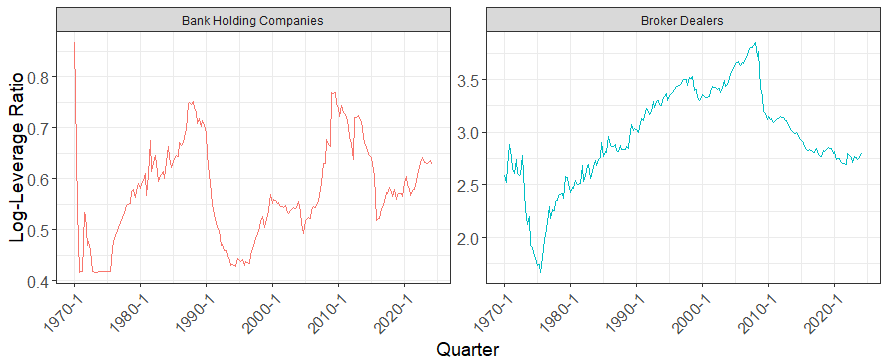
\includegraphics[width=\textwidth]{Log_Leverage.png}
		\label{fig:log_leverage}
		\floatfoot{\textit{Note:} Source: own creation.}
	\end{figure}
	
	And figure \ref{fig:aggregate_nws_ll} displays the aggregate log leverage as well as the net worth share of bank holding companies.
	
	\begin{figure}[H]
 		\caption{Aggregate Log Leverage and Net Worth share of Bank Holding Companies}
 		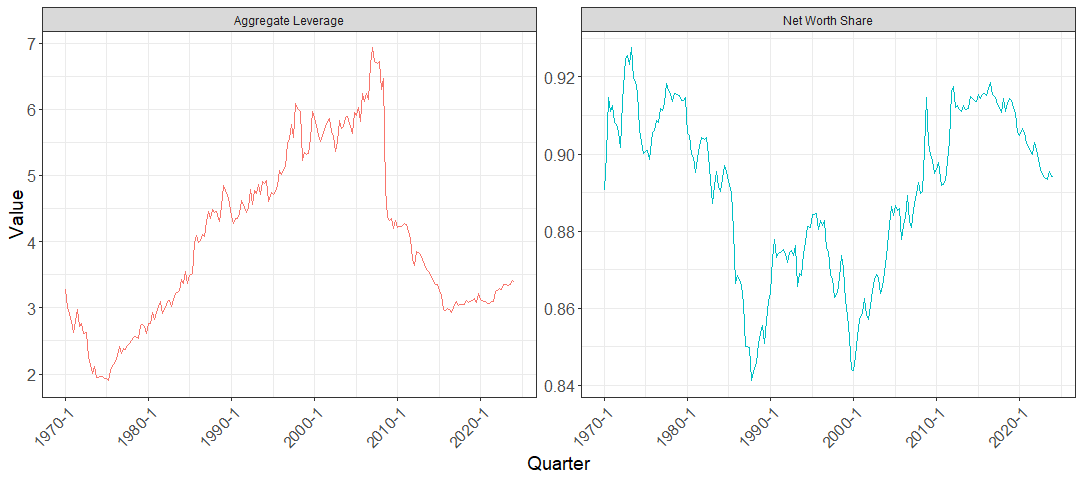
\includegraphics[width=\textwidth]{Aggregate.png}
 		\label{fig:aggregate_nws_ll}
 		\floatfoot{\textit{Note:} Source: own creation.}
 	\end{figure}
	
	

\section{Empirical Results}

	\subsection{Parameter Estimation Results}

	What should be answered here:
	
	* What are the key parameter estimates?
	* What are the key parameter estimates' standard errors?
	* What are the key parameter estimates' confidence intervals?
	* What are the key parameter estimates' p-values?
	* Are the parameters in line with the literature?
	* How do the parameters compared to the literature?
	* Display the parameter estimates in a table.
	* Display the highly non-linear relationship between the parameters in a plot (page 17 of paper).
	* Compare Parameter Results between using the efficient GMM weighing matrix and the identity matrix.


	\subsection{Problems in the Empirical Estimation Process}

		\subsubsection{Parameter Behavior with major Economic Indicators} 

		* How do the parameters behave compared move with the GDP and major economic indicators?

		\subsubsection{Fama-MacBeth Regressions}

		* Perform linear tests and how well the model explains the asset returns.
		* Explain how Fama-MacBeth Regressions work.
		* Perform Fama-MacBeth Regressions and explain the results.




		\subsubsection{Model Robustness}

		* With respect to Covid-19 Crisis.
		* With Respect to out of sample performance (page 31 of the paper).


\section{Conclusion}

What should be answered here:

* What are the key results?
* What are the key implications?
* What are the key limitations of my paper and what could be elaborated on?
* What are the key future research directions?
* Are the results of my analysis in line with the literature, especially with the paper I am re-building on?

		
		
		

\newpage

		
\bookmarksetup{startatroot} %next section in pdf document on top level
\addcontentsline{toc}{section}{Bibliography}\label{sec:references}
\renewcommand{\refname}{Bibliography}
\begin{thebibliography}{99}
	
	
	
	\bibitem[Ager et al. (2009)]{Ager09}
	\textbf{Ager, P.; Kappler, M. \& Osterloh, S. (2009):}
	"The accuracy and efficiency of the Consensus Forecasts: A further application and extension of the pooled approach,"
	\emph{International Journal of Forecasting}, 25(1), 167--181.
	
	\bibitem[Artis (1996)]{Artis96}
	\textbf{Artis, M. J. (1996):}
	"How Accurate Are the Imf's Short-Term Forecasts? Another Examination of the World Economic Outlook,"
	\emph{IMF Working Papers}, 1996(89), 1--73.\\
	\url{https://doi.org/10.5089/9781451851250.001}
	
	\bibitem[Andreou et al. (2013)]{Andre13}
	\textbf{Andreou, E.; Ghysels, E. \& Kourtellos, A. (2013):}
	"Should macroeconomic forecasters use daily financial data and how?,"
	\emph{Journal of Business \& Economic Statistics}, 31(2), 240--251.	
	
	\bibitem[Batchelor and Dua(1991)]{Batchelor_Dua}
	\textbf{Batchelor, R. \& Dua, P. (1991):}
	"Blue Chip Rationality Tests,"
	\emph{Journal of Money, Credit and Banking}, 23(4), 692--705.
	
	\bibitem[Batchelor (2007)]{Batchelor(2007)}
	\textbf{Batchelor, R. (2007):}
	"Bias in macroeconomic forecasts,"
	\emph{International Journal of Forecasting}, 23(2), 189--203.
	
	\bibitem[Bonham and Cohen (2001)]{Bonham01}
	\textbf{Bonham, C. S. \& Cohen, R. H. (2001):}
	"To aggregate, pool, or neither: Testing the rational-expectations hypothesis using survey data,"
	\emph{Journal of Business \& Economic Statistics}, 19(3), 278--291.
	
	\bibitem[Carroll (2003)]{Carroll(2003)}
	\textbf{Carroll, C. D. (2003):}
	"Macroeconomic Expectations of Households and Professional Forecasters,"
	\emph{The Quarterly Journal of Economics}, 118(1), 269--298.
	
	\bibitem[Cho (2002)]{Cho(2002)}
	\textbf{Cho, D. W. (2002):}
	"Do revisions improve forecasts?,"
	\emph{International Journal of Forecasting}, 18(1), 107--115.
	
	\bibitem[Clements and Galvão (2008)]{Clements(2008)}
	\textbf{Clements, M. P. \& Galvão, A. B. (2008):}
	"Macroeconomic forecasting with mixed-frequency data: Forecasting output growth in the United States,"
	\emph{Journal of Business \& Economic Statistics}, 26(4), 546--554.
	
	\bibitem[Clements and Hendry (2002)]{Clements_Hendry}
	\textbf{Clements, M. P. \& Hendry, D. F. (2002):}
	"An Overview of Economic Forecasting,"
	in: Clements, M.P. \& Hendry, D.F. (Edt.):
	\emph{A Companion to Economic Forecasting}, 1--18, Blackwell Publishing Ltd, Cornwall.
	
	\bibitem[Croushore and Stark (2019)]{Croushore_Stark(2019)}
	\textbf{Croushore, D. \& Stark, T. (2019):}
	"Fifty Years of the Survey of Professional Forecasters,"
	\emph{Economic Insights}, 4(4), 1--11.
	
	\bibitem[Deschamps and Ioannidis (2014)]{Deschamps_Ioannidis}
	\textbf{Deschamps, B. \& Ioannidis, C. (2014):}
	"The Efficiency of Multivariate Macroeconomic Forecasts,"
	\emph{The Manchester School}, 82(5), 509--523.
	
	\bibitem[Dovern and Weisser (2008)]{Dovern08}
	\textbf{Dovern, J. \& Weisser, J. (2008):}
	"Are they really rational? Assessing professional macro-economic forecasts from the G7-countries,"
	\emph{Kiel Working Paper (No. 1447)}, 1--45.\\
	\url{http://hdl.handle.net/10419/24842}
	
	\bibitem[Dovern and Weisser (2011)]{Dovern_Weisser(2011)}
	\textbf{Dovern, J. \& Weisser, J. (2011):}
	"Accuracy, unbiasedness and efficiency of professional macroeconomic forecasts: An empirical comparison for the G7,"
	\emph{International Journal of Forecasting}, 27(2), 452--465.
	
	\bibitem[Elliott and Timmermann (2008)]{Elliott_Timmermann(2008)}
	\textbf{Elliott, G. \& Timmermann, A. (2008):}
	"Economic Forecasting,"
	\emph{Journal of Economic Literature}, 46(1), 3--56.
	
	\bibitem[Elliott et al. (2005)]{Elliott_etal(2005)}
	\textbf{Elliott, G.; Timmermann, A. \& Komunjer, I. (2005):}
	"Estimation and Testing of Forecast Rationality under Flexible Loss,"
	\emph{The Review of Economic Studies}, 72(4), 1107--1125.
	
	\bibitem[Fama (1965)]{Fama}	
	\textbf{Fama, E. F. (1965):}
	"The behavior of stock-market prices,"
	\emph{Journal of Business}, 38(1), 34--105.
	
	\bibitem[Fildes Fitzgerald (1983)]{Fildes_Fitzgerald}
	\textbf{Fildes, R. \& Fitzgerald, M. D. (1983):}
	"The Use of Information in Balance of Payments Forecasting,"
	\emph{Economica}, 50(199), 249--258.
	
	\bibitem[Fildes and Stekler (2002)]{Fildes_Stekler}
	\textbf{Fildes, R. \& Stekler, H. O. (2002):}
	"The state of Macroeconomic Forecasting,"
	\emph{Journal of Macroeconomics}, 24(4), 435--468.
	
	\bibitem[Fintzen and Stekler (1999)]{Fintzen_Stekler}
	\textbf{Fintzen, D.\& Stekler, H. O. (1999):}
	"Why did forecasters fail to predict the 1990 recession?,"
	\emph{International Journal of Forecasting}, 15(3), 309--323.
	
	\bibitem[Franses et al. (2011)]{Franses_2011}
	\textbf{Franses, P. H.; Kranendonk, H. C. \& Lanser, D. (2011):}
	"One model and various experts: Evaluating Dutch macroeconomic forecasts,"
	\emph{International Journal of Forecasting}, 27(2), 482--495.
	
	\bibitem[Franses et al. (2014)]{Franses14}
	\textbf{Franses, P. H.; McAleer, M. \& Legerstee, R. (2014):}
	"Evaluating macroeconomic forecasts: a concise review of some recent developments,"
	\emph{Journal of Economic Surveys}, 28(2), 195--208.
	
	\bibitem[Gallo et al. (2002)]{Gallo02}
	\textbf{Gallo, G. M.; Granger, C. W. J. \& Jeon, Y. (2002):}
	"Copycats and Common Swings: The Impact of the Use of Forecasts in Information Sets,"
	\emph{IMF Staff Papers}, 2002(2), 4--21.
	
	\bibitem[Geweke and Amisano (2011)]{Geweke11}
	\textbf{Geweke, J. \& Amisano, G. (2011):}
	"Optimal prediction pools,"
	\emph{Journal of Econometrics}, 164(1), 130--141.
	
	\bibitem[Goodwin (2000a)]{Goodwin00a}
	\textbf{Goodwin, P. (2000a):}
	"Improving the voluntary integration of statistical forecasts and judgment,"
	\emph{International Journal of Forecasting}, 16(1), 85--99.
	
	\bibitem[Goodwin (2000b)]{Goodwin00b}
	\textbf{Goodwin, P. (2000b):}
	"Correct or combine? Mechanically integrating judgmental forecasts with statistical methods,"
	\emph{International Journal of Forecasting}, 16(2), 261--275.
	
	\bibitem[Goodwin (2005)]{Goodwin(2005)}
	\textbf{Goodwin, P. (2005):}
	"How to Integrate Management Judgment with Statistical Forecasts,"
	\emph{Foresight: The International Journal of Applied Forecasting}, (1), 8--12.
	
	\bibitem[Heilemann and Stekler (2013)]{Heilemann_Stekler}
	\textbf{Heilemann, U. \& Stekler, H. O. (2013):}
	"Has The Accuracy of Macroeconomic Forecasts for Germany Improved?,"
	\emph{German Economic Review}, 14(2), 235--253.
	
	\bibitem[Holden and Peel (1990)]{HP90}
	\textbf{Holden, K. \& Peel, D. (1990):}
	"On Testing for Unbiasedness and Efficiency of Forecasts,"
	\emph{The Manchester School of Economic \& Social Studies}, 58(2), 120--127.
	
	\bibitem[Holden et al. (1990)]{Holdenetal90}
	\textbf{Holden, K.; Peel, D. A. \& Thompson, J. L. (1990):}
	"Combining forecasts,"
	in: Holden, K.; Peel, D.A. \& Thompson J.L. (Edt.):
	\emph{Economic forecasting: an introduction}, 85--109, Cambridge University Press.
	
	\bibitem[Isiklar et al. (2006)]{Isiklar06}
	\textbf{Isiklar, G.; Lahiri, K. \& Loungani, P. (2006):}
	"How quickly do forecasters incorporate news? Evidence from cross-country surveys,"
	\emph{Journal of applied econometrics}, 21, 703--725.
	
	\bibitem[Lamont (2002)]{Lamont02}
	\textbf{Lamont, O. A. (2002):}
	"Macroeconomic forecasts and microeconomic forecasters,"
	\emph{Journal of economic behavior \& organization}, 48(3), 265--280.
	
	\bibitem[Laster et al. (1999)]{Laster99}
	\textbf{Laster, D.; Bennett, P. \& Geoum, I. S. (1999):}
	"Rational bias in macroeconomic forecasts,"
	\emph{The Quarterly Journal of Economics}, 114(1), 293--318.
	
	\bibitem[Lawrence et al. (2006)]{Lawrence06}
	\textbf{Lawrence, M.; Goodwin, P.; O'Connor, M. \& Önkal, D. (2006):}
	"Judgmental forecasting: A review of progress over the last 25 years,"
	\emph{International Journal of Forecasting}, 22(3), 493--518.
	
	\bibitem[Loungani (2001)]{Loungani01}
	\textbf{Loungani, P. (2001):}
	"How accurate are private sector forecasts? Cross-country evidence from consensus forecasts of output growth,"
	\emph{International Journal of Forecasting}, 17(3), 419--432.
	
	\bibitem[McNees (1990)]{McNees90}
	\textbf{McNees, S. K. (1990):}
	"The role of judgment in macroeconomic forecasting accuracy,"
	\emph{International Journal of Forecasting}, 6(3), 287--299.
	
	\bibitem[Meyler and Rubene (2009)]{Meyler09}
	\textbf{Meyler, A. \& Rubene, I. (2009):}
	"Results of a special questionnaire for participants in the ECB Survey of Professional Forecasters (SPF),"
	\emph{European Central Bank Economic Bulletin}, 1--16.\\
	\url{https://mpra.ub.uni-muenchen.de/20751/}
	
	\bibitem[Mincer and Zarnowitz (1969)]{MZ69}
	\textbf{Mincer, J. A. \& Zarnowitz, V. (1969):}
	"The Evolution of Economic Forecasts,"
	\emph{Economic Forecasts and Expectations: Analysis of Forecasting Behavior and Performance}, 3--43.
	
	\bibitem[Nordhaus (1987)]{Nordhaus87}
	\textbf{Nordhaus, W. (1987):}
	"Forecasting Efficiency: Concepts and Applications,"
	\emph{The Review of Economics and Statistics}, 69(4), 667--674.
	
	\bibitem[Oeller and Barot (2000)]{Oeller00}
	\textbf{Öller, L. \& Barot, B. (2000):}
	"The accuracy of European growth and inflation forecasts,"
	\emph{International Journal of Forecasting}, 16(3), 293--315.
	
	\bibitem[Patton and Timmermann (2011)]{Patton11}
	\textbf{Patton, A. J. \& Timmermann, A. (2011):}
	"Predictability of Output Growth and Inflation: A Multi-Horizon Survey Approach,"
	\emph{Journal of Business \& Economic Statistics}, 29(3), 397--410.
	
	\bibitem[Schnader and Stekler (1998)]{Schander98}
	\textbf{Schnader, M. H.\& Stekler, H. O. (1998):}
	"Sources of turning point forecast errors,"
	\emph{Applied Economics Letters}, 5(8), 519--521.
	
	\bibitem[Scotese (1994)]{Scotese94}
	\textbf{Scotese, C. A. (1994):}
	"Forecast smoothing and the optimal under-utilization of information at the federal reserve,"
	\emph{Journal of Macroeconomics}, 16(4), 653--670.
	
	\bibitem[Stark (2010)]{Stark10}
	\textbf{Stark, T. (2010):}
	"Realistic Evaluation of Real-Time Forecasts in the Survey of Professional Forecasters,"
	\emph{Federal Reserve Bank of Philadelphia Research Rap}, 1, 1--20.
	
	\bibitem[Stark (2013)]{Stark13}
	\textbf{Stark, T. (2013):}
	"SPF panelists' forecasting methods: A note on the aggregate results of a November 2009 special survey,"
	\emph{Federal Reserve Bank of Philadelphia}, 1--11.
	
	\bibitem[Stekler (2002)]{Stekler02}
	\textbf{Stekler, H. O. (2002):}
	"The rationality and efficiency of individuals´ forecasts,"
	in: Clements, M.P. \& Hendry, D.F. (Edt.):
	\emph{A Companion to Economic Forecasting}, 222--240, Blackwell Publishing Ltd, Cornwall.
	
	\bibitem[Stekler (2007)]{Stekler07}
	\textbf{Stekler, H. O. (2007):}
	"The future of macroeconomic forecasting: Understanding the forecasting process,"
	\emph{International Journal of Forecasting}, 23(2), 237--248.
	
	\bibitem[Theil (1966)]{Theil66}
	\textbf{Theil, H. (1966):}
	"Applied economic forecasting,"
	\emph{Economic Forecasting}.	
	
	\bibitem[Welch and Goyal (2008)]{Welch08}
	\textbf{Welch, I. \& Goyal, A. (2008):}
	"A Comprehensive Look at The Empirical Performance of Equity Premium Prediction,"
	\emph{Review of Financial Studies}, 21(4), 1455--1508.
	
	\bibitem[Zarnowitz (1985)]{Zarno85}
	\textbf{Zarnowitz, V. (1985):}
	"Rational expectations and macroeconomic forecasts,"
	\emph{Journal of Business \& Economic Statistics}, 3(4), 293--311.
	
	\bibitem[Zarnowitz and Braun (1993)]{Zarno93}
	\textbf{Zarnowitz, V. \& Braun, P. (1993):}
	"Twenty-two years of the NBER-ASA quarterly economic outlook surveys: aspects and comparisons of forecasting performance,"
	in: Stock, J.H. \& Watson, M.W. (Edt.):
	\emph{Business cycles, indicators, and forecasting}, 11--94, University of Chicago Press.
	
	\bibitem[Zarnowitz and Lambros (1987)]{Zarno87}
	\textbf{Zarnowitz, V. \& Lambros, L. A. (1987):}
	"Consensus and uncertainty in economic prediction,"
	\emph{Journal of Political economy}, 95(3), 591--621.
	
	
	
\end{thebibliography}

\cleardoublepage\phantomsection %corrects hyperlink in pdf document
\addcontentsline{toc}{section}{Appendix}
\setcounter{table}{0}\setcounter{figure}{0}\setcounter{equation}{0}\setcounter{subsection}{0}
\renewcommand{\thesubsection}{A.\arabic{subsection}}
\renewcommand{\thetable}{A\arabic{table}}
\renewcommand{\thefigure}{A\arabic{figure}}
\renewcommand{\theequation}{A\arabic{equation}}

\section*{Appendix}


		
		
		
		
		
		\clearpage
		\thispagestyle{empty}\mbox{}
		\clearpage
		

	\end{document}	